\documentclass[a4paper,12pt]{article}

\usepackage[utf8]{inputenc}
\usepackage[T1]{fontenc}
\usepackage[spanish]{babel}

\usepackage{graphicx}
\usepackage{listings}
\usepackage{amsmath}
\usepackage{geometry}
\usepackage{float}

\usepackage[hidelinks]{hyperref}
\def\UrlBreaks{\do\/\do-}

\geometry{margin=2.5cm}

\title{Proyecto RAG: Asistente de Trámites para Familias con Miembros con Autismo en Andalucía}
\author{Cristóbal Navas Mesa}
\date{}

\begin{document}

\begin{titlepage}
    \centering
    \vspace*{1.5cm}
    % \includegraphics[width=0.4\textwidth]{ruta/al/logo.png}\par\vspace{1cm}
    {\bfseries\Huge Proyecto RAG: \par}
    {\bfseries\Huge Asistente de Trámites para Familias \par}
    {\bfseries\Huge con Miembros con Autismo en Andalucía \par}
    \vspace{2cm}
    {\Large \textsc{Cristóbal Navas Mesa} \par}
    \vspace{1cm}
    \rule{\linewidth}{0.5mm} \\[0.4cm]
    {\large \today \par}
    \rule{\linewidth}{0.5mm} \\[1.5cm]
    \vfill
    \large{Memoria del Proyecto\par}
    \vspace{0.5cm}
    \vfill
\end{titlepage}

\newpage

\tableofcontents
\newpage

\begin{abstract}
Este documento presenta el desarrollo de un sistema Retrieval-Augmented Generation (RAG) como asistente para familias con miembros con Trastorno del Espectro Autista (TEA) en Andalucía. El sistema facilita la consulta de normativa administrativa, ayudas y trámites mediante técnicas de procesamiento de lenguaje natural e inteligencia artificial.
\end{abstract}

\section{Introducción}

\subsection{Descripción general}
Las familias con hijos o hijas diagnosticados con Trastorno del Espectro Autista (TEA) en Andalucía enfrentan numerosos desafíos para acceder y comprender los trámites y recursos disponibles. La dispersión de la información en portales web múltiples, documentos en formato PDF, BOJA y guías oficiales dificulta el acceso sencillo y rápido a información actualizada y relevante. Este proyecto nace de la necesidad de crear una herramienta tecnológica que facilite la navegación, búsqueda y comprensión de conceptos normativos y procedimentales, proporcionando un acceso centralizado y amigable mediante técnicas avanzadas de procesamiento del lenguaje natural e inteligencia artificial, concretamente a través de un sistema Retrieval-Augmented Generation (RAG).

\subsection{Objetivos}
\begin{itemize}
    \item Recopilar y organizar documentación normativa y de procedimiento relevante para familias con miembros con TEA en Andalucía.
    \item Procesar documentos en formatos diversos para convertirlos en texto plano limpio.
    \item Dividir la información en fragmentos o \textit{chunks} para su posterior vectorización.
    \item Crear una base de datos semántica con embeddings para búsqueda de información.
    \item Implementar un sistema de búsqueda y generación de respuestas mediante modelos de lenguaje.
    \item Desarrollar una interfaz sencilla de uso para los usuarios finales.
    \item Realizar pruebas y validación de la calidad y utilidad del sistema.
\end{itemize}

\section{Alcance del Proyecto}
El sistema se centra en los trámites y recursos para familias con miembros con TEA en Andalucía, incluyendo pero no limitado a:
\begin{itemize}
    \item Reconocimiento de grado de discapacidad.
    \item Acceso a atención temprana (0-6 años).
    \item Trámites relacionados con escolarización y NEAE/NNEE.
    \item Ayudas económicas, prestaciones y apoyos a la autonomía.
    \item Recursos específicos de asociaciones y federaciones de autismo.
\end{itemize}

\section{Metodología y Desarrollo}

\subsection{Fases del proyecto}

\begin{enumerate}
    \item \textbf{Búsqueda y recopilación de normativa y procedimientos}: 
    Se localizaron fuentes oficiales de información como Junta de Andalucía, BOJA, portales educativos y sociales. Se seleccionaron leyes, decretos, guías, documentos explicativos, Preguntas Frecuentes (FAQs), descargándolos y organizándolos en estructura clara.

    \item \textbf{Conversión y limpieza de información}:
    Para asegurar la calidad y uniformidad de los datos, se aplicaron técnicas automatizadas y manuales de extracción y preprocesamiento. Se usaron librerías Python especializadas para extraer texto de PDFs heterogéneos, normalizando codificaciones y eliminando metadatos innecesarios. Se implementaron reglas heurísticas para detectar y eliminar contenido repetitivo, encabezados, pie de página y numeración, garantizando textos limpios y coherentes para las fases posteriores.

    \item \textbf{Definición de estrategia de chunking}: 
    Segmentación de los textos en fragmentos adecuados para indexar. Se usó un tamaño aproximado de 500 caracteres con solapamiento de 100 caracteres para evitar corte de ideas importantes. Se asociaron metadatos básicos con cada chunk tales como fuente, título, sección y URL.

    \item \textbf{Creación de embeddings y almacenamiento}: 
    La selección del modelo de embeddings se fundamentó en su eficacia para captar la semántica en español. Se optó por modelos basados en Sentence Transformers adaptados al dominio normativo-social. Los embeddings generados se almacenaron en ChromaDB, una base de datos vectorial de alto rendimiento que facilita búsquedas semánticas rápidas y relevantes mediante técnicas de similitud vectorial.

    \item \textbf{Implementación del sistema RAG}: 
    Se desarrolló la capa que combina la búsqueda semántica en el vector store y la generación de respuestas naturales con un modelo de lenguaje de gran tamaño (LLM local).

    \item \textbf{Desarrollo de la interfaz}: 
    Creación de una aplicación web con Flask que proporciona una experiencia usuario amigable, permitiendo consultas en lenguaje natural y visualización enriquecida con fuentes documentales.

    \item \textbf{Pruebas y evaluación}: 
    Elaboración de preguntas de prueba, así como análisis cualitativo y cuantitativo de la pertinencia y claridad de las respuestas generadas.
\end{enumerate}

\subsection{Arquitectura del sistema}

El sistema consta de:
\begin{itemize}
    \item \textbf{Pipeline de procesamiento de datos}: Módulos para extracción, limpieza, chunking y embedding.
    \item \textbf{Base vectorial}: ChromaDB donde se almacenan embeddings y metadatos.
    \item \textbf{Backend LLM}: Servicio local LM Studio que genera respuestas.
    \item \textbf{Interfaz web}: Aplicación Flask para interacción usuario-sistema.
\end{itemize}

\paragraph{Diagrama de arquitectura (ejemplo conceptual)}
\vspace{0.5cm}
\noindent
\begin{figure}[H]
  \centering
  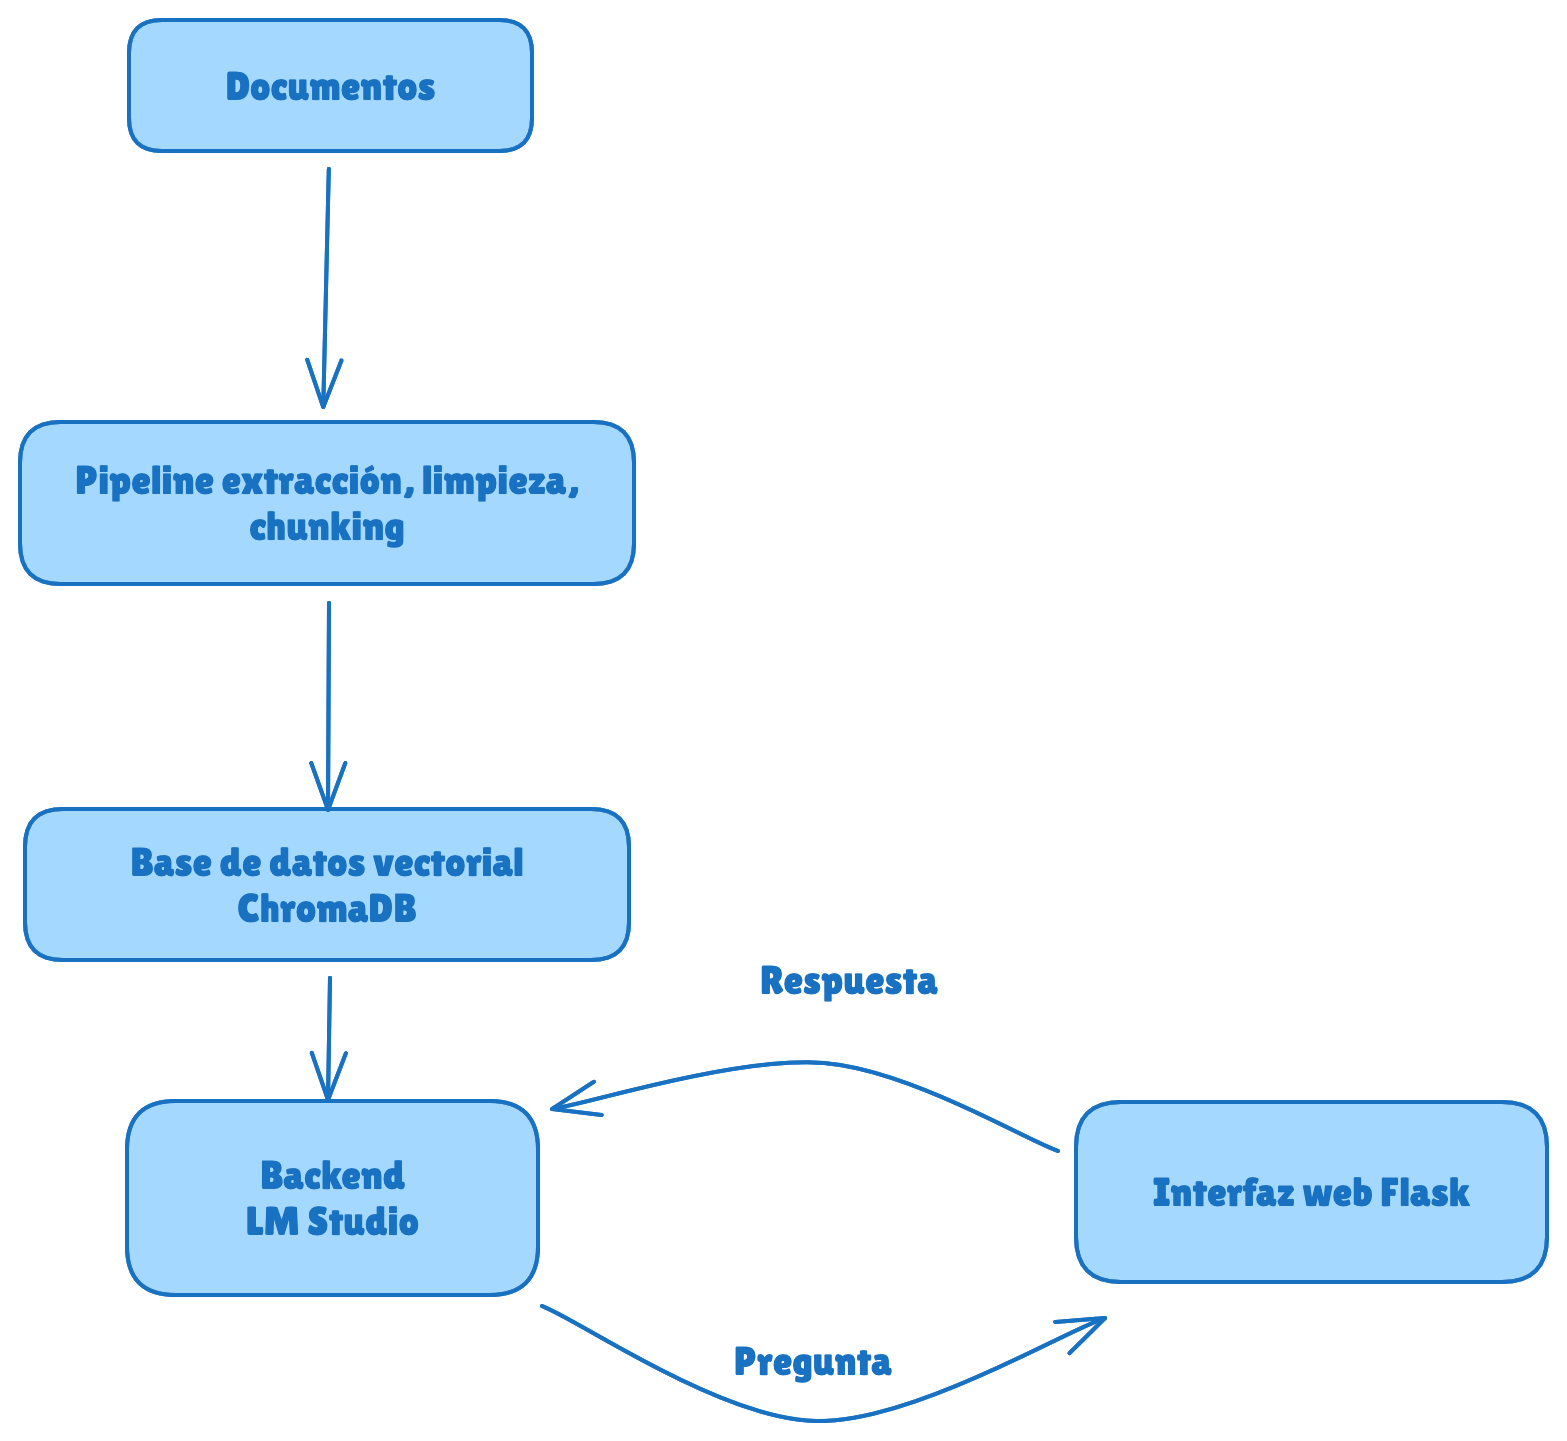
\includegraphics[width=0.7\textwidth]{diagrama.png}
  \caption{Arquitectura del sistema RAG desarrollado}
\end{figure}

\vspace{1cm}

\section{Herramientas y tecnologías}

\begin{itemize}
    \item \textbf{Python} con librerías como requests, Flask, chromadb para la orquestación y procesamiento.
    \item \textbf{LM Studio}: Modelo de lenguaje local utilizado para la generación y respuesta.
    \item \textbf{ChromaDB}: Base de datos vectorial para almacenamiento y búsqueda semántica eficiente.
    \item \textbf{Tailwind CSS}: Framework CSS para diseño responsivo y accesible de la interfaz web.
    \item \textbf{Librerías para extracción y limpieza}: Herramientas para convertir PDFs/HTML a texto y normalizar datos.
\end{itemize}

\section{Resultados}

\subsection{Funcionamiento del pipeline}

El pipeline ha sido capaz de procesar una amplia colección de documentos normativos sobre TEA en Andalucía, limpiando, segmentando y generando embeddings eficientes para búsqueda semántica. Esto ha permitido construir una base documental accesible para sistemas de generación de respuestas.

\subsection{Interfaz de usuario}

La interfaz web permite consultas en lenguaje natural, mantiene un historial de preguntas y respuestas, y muestra referencias legibles a fuentes documentales. Su diseño oscuro y responsivo mejora la experiencia de usuario y accesibilidad.

\subsection{Ejemplos de preguntas y respuestas}

Se validaron preguntas relacionadas con trámites destacando:

\begin{itemize}
    \item Procedimientos para solicitar atención temprana.
    \item Ayudas económicas disponibles para personas con TEA.
    \item Pasos para el reconocimiento de discapacidad.
\end{itemize}

Las respuestas generadas incluyen fragmentos normativos precisos que facilitan la comprensión y la confianza del usuario.

\section{Evaluación y pruebas}

Se definió un conjunto de preguntas típicas para familias con TEA y se analizaron respuestas en términos de relevancia, precisión y claridad. Se llevó a cabo una evaluación cualitativa con expertos y usuarios.

\section{Limitaciones y riesgos}

El sistema depende de la calidad de la base documental y requiere actualización constante. Existen riesgos relacionados con la interpretación incorrecta por parte del usuario final y limitaciones del modelo de lenguaje.

\section{Impacto social}

Este sistema apoya la inclusión, autonomía e información de familias TEA, facilitando el acceso a recursos públicos y legales de forma comprensible.

\section{Conclusiones y trabajo futuro}

\subsection{Conclusiones}

El proyecto ha demostrado la viabilidad de usar técnicas RAG en el ámbito social para mejorar el acceso a la información a colectivos vulnerables.

\subsection{Trabajo futuro}

Se plantea incorporar streaming en las respuestas, APIs REST para integración multiplataforma, ampliación documental y procesamiento multilingüe.

\section{Consideraciones éticas y legales}

El sistema es un apoyo informativo y no reemplaza asesoramiento profesional. Es esencial mantener un lenguaje claro, respetuoso y la actualización normativa.

\section{Referencias}

\begin{itemize}
    \item Ley 1-2023 Atención Temprana (Junta de Andaluca)
    \item Ley 4-2017 Derechos Discapacidad (Real Patronato de la Discapacidad)
    \item Decreto 147-2002 Atención Educativa NEAE (Junta de Andalucía)
    \item Solicitud Grado Discapacidad (Junta de Andalucía)
    \item Derechos y Prestaciones Discapacidad (Junta de Andalucía)
\end{itemize}


\end{document}
